\partsintesi{Síntesi de la Part III}{Geometria en el pla}
 
\begin{mylist}
	
 \exer[2] \begin{minipage}[t]{0.6\textwidth}
 	Donats els vectors de la figura calcula:
 \begin{tasks}(3)
 	\task $|\vec u|$
 	\task $-2\vec u + 3\vvec$
 	\task $2\vec u \cdot (\vec u + \vvec)$	
 \end{tasks}
\end{minipage}
\begin{minipage}{0.4\textwidth}
	\begin{center}
	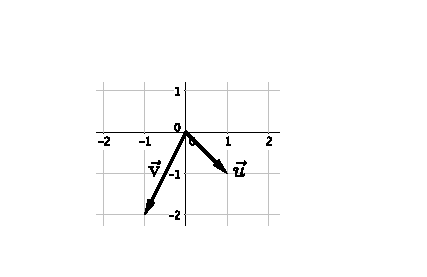
\includegraphics[width=0.8\textwidth]{img-10-bloc3/bloc3-vectors}
	\end{center}
\end{minipage}
\answers{a) $|\vec u|=\sqrt{2}$
	b) $-2\vec u + 3\vvec=(-5,-4)$
	c) $2\vec u \cdot (\vec u + \vvec)=6$}

\exer[2] Determina el valor de $a$ perquè els vectors $(1,3)$ i $(6,a)$ siguin ortogonals.
\answers{ $a=-2$}

\exer[2] Donats els vectors $\vec u(-1,0)$ i $\vvec(1,2)$
 \begin{tasks}
	\task Expressa el vector $\vec w(4,6)$ com a combinació lineal de $\vec u$ i $\vec v$.
	
	 Recorda: $\vec w= m \vec u + n \vvec$.
	\task Calcula l'angle que formen  $\vec u$ i $\vec v$.
\end{tasks}
\answers{a) $m=-1$, $n=3$   b) $116.57^\circ$}

\exer[2] Determina les components d'un vector $(x,y)$ sabent que és unitari i que forma un angle de $60^\circ$ amb el vector $(2,0)$.
\answers{$(\frac{1}{2}, \frac{\sqrt{3}}{2})$}

\exer[2] Determina el valor de $y$ perquè els punts $A(0,1)$, $B(-1,4)$ i $C(3,y)$ estiguin alineats.
\answers{$y=-8$}

\exer[2] Troba en forma paramètrica i general l'equació de la recta que passa per $P(0,3)$ i és perpendicular a la recta $s: \, \dfrac{x+1}{2}=\dfrac{y-1}{-1}$.
\answers{Paramètriques $\left\{\begin{array}{l} x=0+1t \\ y=3+2t \end{array}\right.$. General $2x-y+3=0$.}

\exer[2]  Es consideren les rectes $r:\, 2x+y-1=0$ i $s:\, kx-y+5=0$. Determina $k$ per a cadascun dels casos següents:
 \begin{tasks}
	\task $r$ i $s$ siguin paral·leles.
	\task $r$ i $s$ es tallin en el punt $P(2,-3)$.
\end{tasks}
\answers{a) $k=-2$.  b) $k=-4$}

\exer[2] Troba el punt simètric de $A(0,0)$ respecte de la recta $r:\, x+y-2=0$.
\answers{$A'(2,2)$}

\exer[2] Troba l'equació de la recta que passa pel punt d'intersecció de les rectes: 

$r:\, 2x-y+1=0$ i $s: \, \dfrac{x+1}{2}=\dfrac{y-5}{2}$ i forma un angle de $45^\circ$ amb la recta $r$.
\answers{El punt d'intersecció és $I(5,11)$ i el pendent de la recta $m'=1/3$. La recta és $y-11=\frac{1}{3}(x-5)$.}

\exer[2] Troba els punts de la recta $y=0$ que disten 3 unitats de la recta $3x-4y=0$.
\answers{$P(\pm 5, 0)$}

\exer[2] Calcula l'àrea del triangle de vèrtexs $A(1,2)$, $B(-1,-2)$ i $C(2,-1)$.
\answers{$Area=5$}

\exer[2] Calcula les mediatrius i les coordenades del circumcentre d'un triangle amb vèrtexs als punts $A(2,-1)$, $B(-5,1)$  i $C(0,3)$.
\answers{Mediatriu AC: $x-2y+1=0$, Mediatriu $AB$: $14x-4y+21=0$, Circumcentre $O(-19/12, -7/24)$}

\exer[2] Troba el centre i el radi de la circumferència $x^2+y^2-2x+6y+6=0$.
\answers{Centre $O(1,-3)$ i radi $R=2$.}

\exer[2] Escriu l'equació de l'el·lipse horitzontal de centre $(0,0)$, sabent que l'excentricitat és $e=4/5$ i que un dels focus és a $F(8,0)$.
\answers{$\frac{x^2}{100}+\frac{y^2}{36}=1$}

\exer[2] Identifica les còniques, calcula'n els seus elements i dibuixa-les:
 \begin{tasks}(2)
	\task $2y^2-12x=0$
	\task $\dfrac{(x-1)^2}{16}-\dfrac{(y+1)^2}{9}=1$
\end{tasks}
\answers{	a) Paràbola vertical amb vèrtex $V(0,0)$, $p=3$, focus $F(0,3/2)$ i directriu la recta $y=-3/2$.
	
	b) Hipèrbola de centre $O(1,-1)$, semieixos $a=4$, $b=3$, semi-distància focal $c=5$. Excentricitat $e=1.25$. Focus a $F'(-4,-1)$, $F(6,-1)$. Asímptotes $y+1=\pm\frac{3}{4}(x-1)$.
	
	\begin{center}
		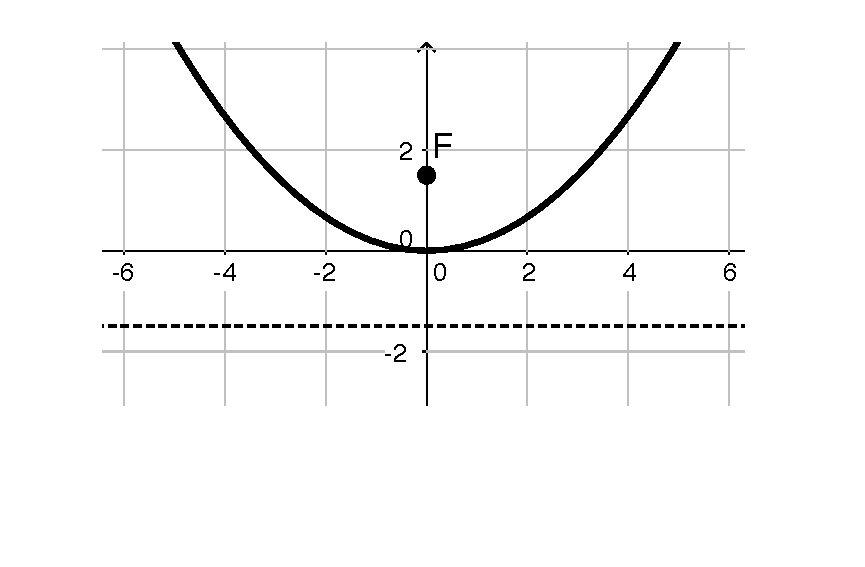
\includegraphics[height=3cm]{img-10-bloc3/bloc3-sol-14a}
		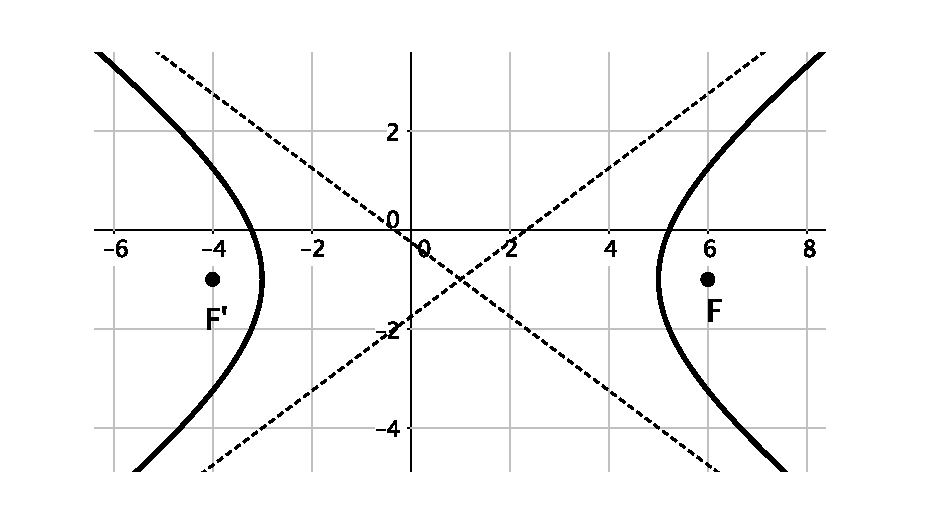
\includegraphics[height=3cm]{img-10-bloc3/bloc3-sol-14b}
	\end{center}
}

\exer[2] Es defineixen l'afeli (periheli) com el punt de l'òrbita d'un planeta que es troba a la màxima (mínima) distància del Sol. Plutó té periheli 29.5 i afeli 49.1 unitats astronòmiques (u.a.), on 1 u.a.=150 milions de quilòmetres. Calcula l'equació de l'òrbita el·líptica i la seva excentricitat. Recorda que el Sol es troba en un dels focus de l'el·lipse.

\answers{$a=39.3$ ua, $c=9.8$ ua, $b=38.06$ ua.  $\dfrac{x^2}{39.3^2}+\dfrac{y^2}{38.06^2}=1$}
\begin{center}
	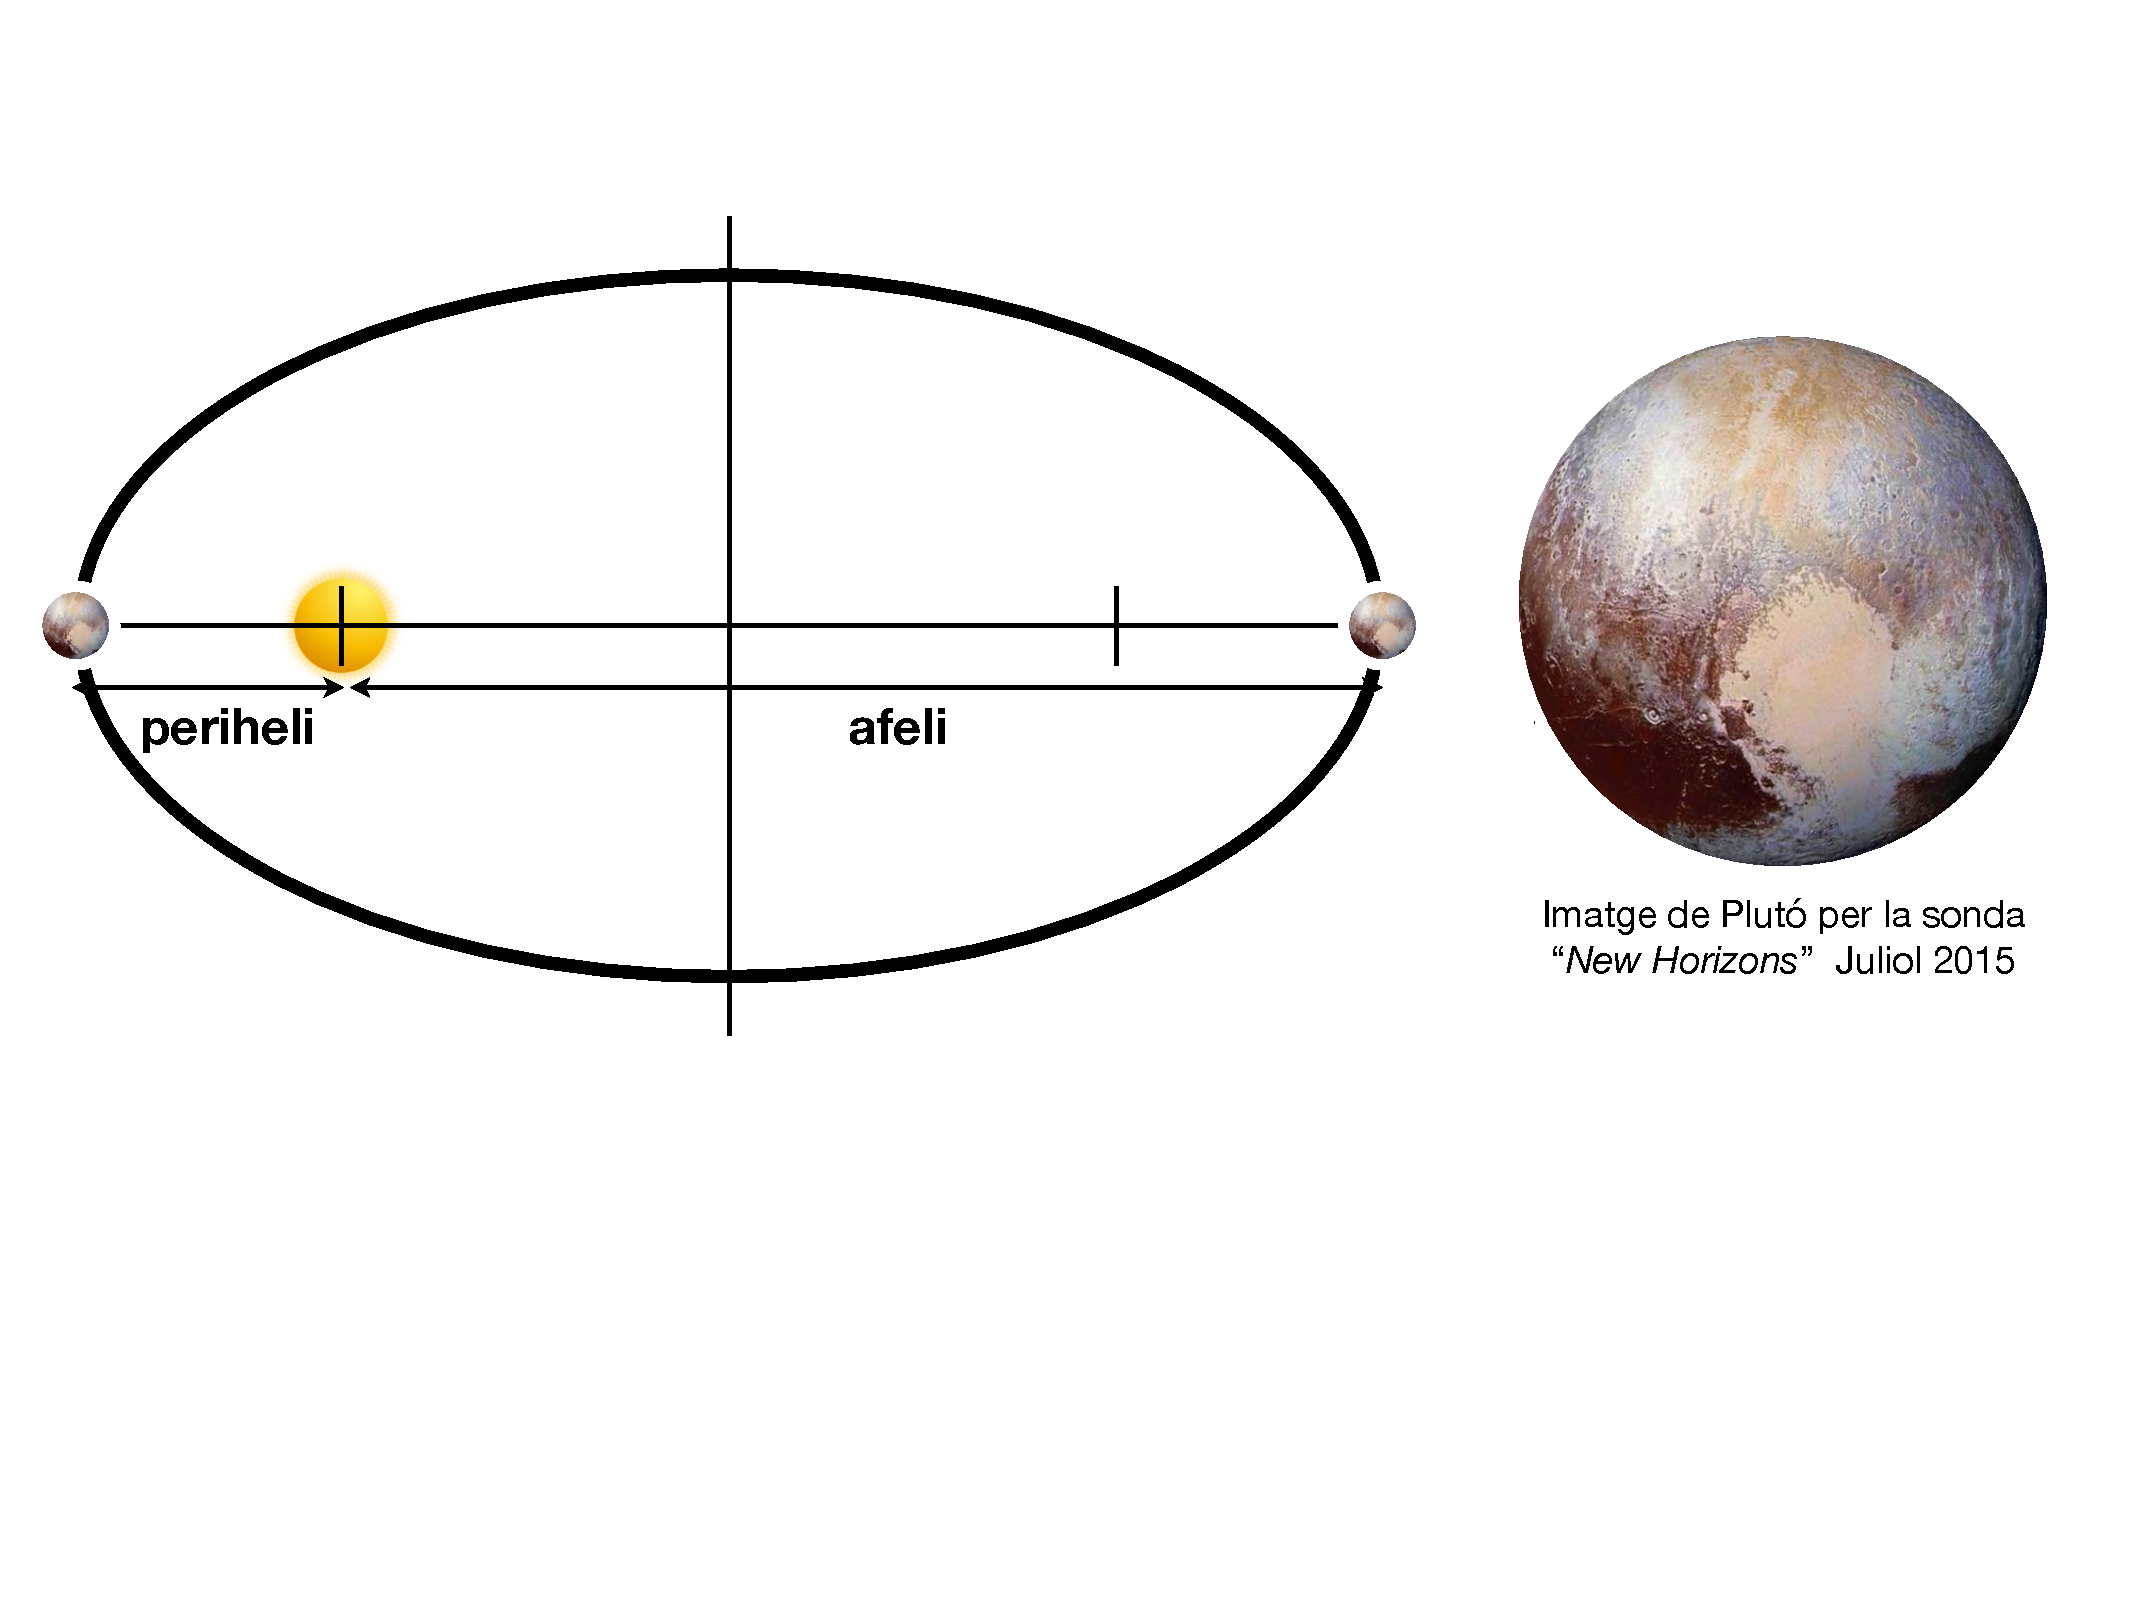
\includegraphics[width=0.6\textwidth]{img-10-bloc3/pluton}
\end{center}

	
\end{mylist}